\documentclass[pdflatex,sn-mathphys-num]{sn-jnl}

\usepackage[utf8]{inputenc}
\usepackage[T1]{fontenc}
\usepackage{amsmath,amssymb,booktabs,graphicx,array,url}
\graphicspath{{../}}

\newcommand{\pir}{\mathrm{PIR}}
\newcommand{\rmpir}{\mathrm{RM\text{-}PIR}}

\let\snabstract\abstract
\let\abstract\relax
\let\endabstract\relax
\NewDocumentEnvironment{abstract}{+b}{\globaldefs=1\snabstract{#1}}{}

\begin{document}

\title[Supplementary Information]{Supplementary Information: RMS-matched Performance Index Rating and EuroLeague team-ledger concordance}
\author*[1]{\fnm{[First name]} \sur{[Family name]}}\email{[corresponding.author@institution.example]}
\author[1]{\fnm{[First name]} \sur{[Family name]}}
\author[1]{\fnm{[First name]} \sur{[Family name]}}
\affil*[1]{\orgdiv{[Department]}, \orgname{[Institution]}, \orgaddress{\city{[City]}, \postcode{[Postcode]}, \country{[Country]}}}

\begin{abstract}
This Supplementary Information contains the extended mathematical derivation, data-provenance record, historical-documentation audit, detailed team rankings, robustness analyses and secondary player diagnostics supporting the main manuscript.
\end{abstract}
\keywords{EuroLeague, RM-PIR, supplementary methods, reproducibility}
\maketitle

\renewcommand{\thesection}{S\arabic{section}}
\renewcommand{\thesubsection}{S\arabic{section}.\arabic{subsection}}
\renewcommand{\thetable}{S\arabic{table}}
\renewcommand{\thefigure}{S\arabic{figure}}
\renewcommand{\theequation}{S\arabic{equation}}

\section{Extended mathematical specification}

\subsection{Official ledger and the points-only degeneracy}

For official player or team row \(u\) in game \(g\), collect the ten unsigned nonpoint counts as
\begin{equation}
\begin{aligned}
\mathbf X_{ug}&=(\mathrm{TR},\mathrm{AST},\mathrm{STL},\mathrm{BLK},\mathrm{FD},
\mathrm{MFG},\mathrm{MFT},\mathrm{TO},\mathrm{BLKA},\mathrm{FC})_{ug}^{\mathsf T},\\
\mathbf s&=(1,1,1,1,1,-1,-1,-1,-1,-1)^{\mathsf T}.
\end{aligned}
\label{eq:s-components}
\end{equation}
Official PIR is \(\pir_{ug}=\mathrm{PTS}_{ug}+\mathbf s^{\mathsf T}\mathbf X_{ug}\). For completed game \(g\), define
\begin{equation}
\mathbf d_g=\mathbf X_{W_g,g}-\mathbf X_{L_g,g},
\qquad
\mathbf x_g=\mathbf s\odot\mathbf d_g,
\qquad
\Delta_g^{\mathrm{PTS}}=\mathrm{PTS}_{W_g,g}-\mathrm{PTS}_{L_g,g}>0.
\label{eq:s-design}
\end{equation}
The official nonpoint and complete contrasts are \(\mathbf x_g^{\mathsf T}\mathbf1_{10}\) and \(\Delta_g^{\mathrm{PTS}}+\mathbf x_g^{\mathsf T}\mathbf1_{10}\), respectively. More generally, a score with signed nonpoint coefficients \(\mathbf c\) has contrast
\begin{equation}
\Delta_g(\mathbf c)=\Delta_g^{\mathrm{PTS}}+\mathbf d_g^{\mathsf T}\mathbf c.
\label{eq:s-general}
\end{equation}
Setting \(\mathbf c=\mathbf0\) makes \(\Delta_g(\mathbf0)=\Delta_g^{\mathrm{PTS}}>0\) in every completed game. Thus points-only scoring is a degeneracy of an unrestricted complete-score ordering criterion. It is not an RM-PIR solution: points are absent from calibration and every raw nonpoint magnitude is constrained away from zero.

\subsection{Eight-group parameterisation}

RM-PIR estimates eight positive raw magnitudes
\begin{equation}
\mathbf a=(a_{\mathrm{TR}},a_{\mathrm{AST}},a_{\mathrm{STL}},a_{\mathrm B},a_{\mathrm F},
a_{\mathrm{MFG}},a_{\mathrm{MFT}},a_{\mathrm{TO}})^{\mathsf T}\in[0.5,1.5]^8.
\label{eq:s-raw}
\end{equation}
The expansion matrix \(\mathbf E\in\{0,1\}^{10\times8}\) implements the block and foul restrictions:
\begin{equation}
\mathbf E\mathbf a=(a_{\mathrm{TR}},a_{\mathrm{AST}},a_{\mathrm{STL}},a_{\mathrm B},a_{\mathrm F},
a_{\mathrm{MFG}},a_{\mathrm{MFT}},a_{\mathrm{TO}},a_{\mathrm B},a_{\mathrm F})^{\mathsf T}.
\label{eq:s-expansion}
\end{equation}
The corresponding fitted nonpoint contrast is \(z_g(\mathbf a)=\mathbf x_g^{\mathsf T}\mathbf E\mathbf a\). Because \(\mathbf E\mathbf1_8=\mathbf1_{10}\), official nonpoint PIR is nested at \(\mathbf a=\mathbf1_8\).

\subsection{Regularised estimation}

With \(\ell_\tau(z)=\log[1+\exp(-z/\tau)]\), the criterion reported in the main paper has gradient
\begin{equation}
\nabla_{\mathbf a}\mathcal L_{\mathcal A}
=-\frac{1}{|\mathcal A|\tau}\sum_{g\in\mathcal A}
\frac{\mathbf E^{\mathsf T}\mathbf x_g}{1+\exp\{z_g(\mathbf a)/\tau\}}
+\frac{2\alpha}{10}\mathbf E^{\mathsf T}(\mathbf E\mathbf a-\mathbf1_{10}).
\label{eq:s-gradient}
\end{equation}
The logistic term is convex. For every candidate \(\alpha>0\), \(\mathbf E\) has full column rank and the ridge Hessian \((2\alpha/10)\mathbf E^{\mathsf T}\mathbf E\) is positive definite. The complete criterion is therefore strictly convex on the convex box and has a unique minimiser. Numerical estimation used the analytic gradient and a bounded limited-memory quasi-Newton method \cite{ByrdEtAl1995}. All 225 inner-grid fits converged, no final fit required fallback estimation, the maximum analytic-versus-finite-difference gradient discrepancy was \(8.91\times10^{-9}\), and final solutions from dispersed starting points differed by no more than \(5.06\times10^{-7}\).

\subsection{Nested selection and locking}

For target season \(Y\), distinct dates in the eligible prior-season window \(\mathcal C_Y\) were ordered chronologically. The earliest 70\% formed \(\mathcal T_Y\), and the remainder formed \(\mathcal V_Y\). Candidate values were
\begin{equation}
\mathcal H=\{1,2,3,5,10\}\times
\{0.001,0.003,0.01,0.03,0.1,0.3,1,3,10\},
\label{eq:s-grid}
\end{equation}
where the coordinates are \(\tau\) and \(\alpha\). Selection first maximised strict validation concordances. Count-equivalent candidates were resolved deterministically by preferring stronger regularisation, smaller \(\tau\), and finally smaller mean validation loss. The selected pair was refitted on all of \(\mathcal C_Y\). This rule yielded the target specifications in Table~\ref{tab:s-models}.

\begin{table}[t]
\caption{Rolling calibration windows and locked model quantities.}
\label{tab:s-models}
\centering
\small
\begin{tabular}{@{}lcrrrr@{}}
\toprule
Target & Calibration seasons & Games & \(\tau\) & \(\alpha\) & \(\gamma\) \\
\midrule
2021--22 & 2020--21 & 328 & 3 & 0.30 & 1.122545 \\
2022--23 & 2020--21 to 2021--22 & 627 & 3 & 0.30 & 1.198911 \\
2023--24 & 2020--21 to 2022--23 & 955 & 5 & 0.01 & 0.994618 \\
2024--25 & 2021--22 to 2023--24 & 958 & 1 & 0.30 & 1.414601 \\
2025--26 & 2022--23 to 2024--25 & 989 & 5 & 0.01 & 1.020537 \\
\bottomrule
\end{tabular}
\end{table}

\subsection{RMS matching, coefficient envelope and complete-score boundary}

For calibration contrasts \(o_g=\mathbf x_g^{\mathsf T}\mathbf1_{10}\) and \(q_{g,Y}=\mathbf x_g^{\mathsf T}\mathbf E\widehat{\mathbf a}_Y\), the main-paper scale factor gives
\begin{equation}
\frac{1}{|\mathcal C_Y|}\sum_{g\in\mathcal C_Y}(\gamma_Yq_{g,Y})^2
=\frac{1}{|\mathcal C_Y|}\sum_{g\in\mathcal C_Y}o_g^2.
\label{eq:s-rms}
\end{equation}
This identity concerns uncentred second moments. Since \(\operatorname{RMS}(v)^2=\operatorname{Var}_{\mathrm{pop}}(v)+\bar v^2\), equal RMS values do not imply equal centred variances when the means differ. Raw bounds and final magnitudes satisfy
\begin{equation}
0.5\leq(\mathbf E\widehat{\mathbf a}_Y)_j\leq1.5
\quad\Longrightarrow\quad
0.5\gamma_Y\leq|c_{j,Y}|\leq1.5\gamma_Y.
\label{eq:s-envelope}
\end{equation}
Because \(\gamma_Y>0\), raw and scaled nonpoint contrasts have the same sign. The complete contrast is
\begin{equation}
\Delta_{g,Y}^{\mathrm{RM}}=\Delta_g^{\mathrm{PTS}}+\gamma_Yz_g(\widehat{\mathbf a}_Y),
\qquad
\Delta_{g,Y}^{\mathrm{RM}}\leq\varepsilon
\Longleftrightarrow
z_g(\widehat{\mathbf a}_Y)\leq\frac{\varepsilon-\Delta_g^{\mathrm{PTS}}}{\gamma_Y}.
\label{eq:s-boundary}
\end{equation}
This explains why scale matching cannot alter nonpoint ordering but can alter complete-score classifications after points are restored.

\subsection{Player/team residual identity}

For team \(t\), game \(g\) and nonpoint field \(j\), define \(r_{tgj}=X_{tgj}-\sum_{i\in t}X_{igj}\), with \(r_{tg,\mathrm{PTS}}\) defined analogously. Substitution into the score gives
\begin{equation}
\rmpir_{tg}^{(Y)}=\sum_{i\in t}\rmpir_{ig}^{(Y)}
+r_{tg,\mathrm{PTS}}+\sum_{j=1}^{10}c_{j,Y}r_{tgj}.
\label{eq:s-additivity}
\end{equation}
The maximum absolute numerical error in this identity was \(4.22\times10^{-14}\). The points residual was zero in all 4,036 team-game rows; other residual actions were kept as explicit team-only contributions rather than assigned to a player.

\section{Data coverage and historical documentation}

\subsection{Season coverage}

\begin{table}[t]
\caption{Included completed games and integrity checks by season. Missing fields and official-PIR reconstruction mismatches were zero in every season.}
\label{tab:s-coverage}
\centering
\small
\begin{tabular}{@{}lrrrrrr@{}}
\toprule
Season & Games & Team rows & Regular & Play-in & Playoffs & Final Four \\
\midrule
2020--21 & 328 & 656 & 306 & 0 & 18 & 4 \\
2021--22 & 299 & 598 & 278 & 0 & 17 & 4 \\
2022--23 & 328 & 656 & 306 & 0 & 18 & 4 \\
2023--24 & 331 & 662 & 306 & 3 & 18 & 4 \\
2024--25 & 330 & 660 & 306 & 3 & 17 & 4 \\
2025--26 & 402 & 804 & 380 & 3 & 16 & 3 \\
\bottomrule
\end{tabular}
\end{table}

Twenty-eight 2021--22 fixtures whose official report had \texttt{played=false} and no completed statistics were excluded from the primary analysis. Their game codes were 156, 167, 171, 172, 182, 184, 239, 240, 243, 244, 248, 250, 253, 258, 261, 262, 266, 267, 271, 276, 280, 283, 284, 289, 294, 299, 300 and 304. No cancellation reason was imputed because the payload did not provide one. The complete exclusion register is supplied as a machine-readable supplementary table.

Game 303 in 2025--26 (Real Madrid--Paris, 5 March 2026) was retained in all 402 primary box-score analyses. It was omitted only from a separate play-by-play possession diagnostic because one malformed-lineup possession was flagged in each team row. That play-by-play diagnostic consequently has 401 games and is not part of the RM-PIR team-ordering result.

\subsection{Documentary evidence for earlier scoring governance}

The Euroleague Basketball Statistics Criteria Manual currently available from the league is version 1.2, validated in September 2025, and states criteria applying from 2024--25 \cite{EuroleagueStatsManual2025}. Two earlier official governance documents were recovered through archived official links:

\begin{itemize}
\item The 2021--22 Euroleague Basketball Bylaws include a Unified Scorers Manual appendix. Article 133.8 requires scorers to follow that appendix and the FIBA Official Basketball Statisticians' Manual, and the post-game procedure provides for video review and correction when a scoresheet does not comply \cite{EuroleagueBylaws2021}.
\item The 2022--23 Euroleague Basketball Bylaws likewise contain a Unified Scorers Manual, refer to the statistics criteria test and require the FIBA manual, with a post-game correction process \cite{EuroleagueBylaws2022}.
\end{itemize}

These records confirm that official statistics before 2024--25 were not collected without documented governance. They do not provide a complete field-by-field change history. We therefore do not claim verified semantic equivalence across all six seasons. Reproducible archive URLs, retrieval dates and file hashes are recorded in \texttt{historical\_criteria\_evidence.md}.

\section{Analysis-decision provenance}

\begin{table}[t]
\caption{Timing of principal analysis decisions. ``Post hoc'' records when a choice was made and limits confirmatory interpretation; it does not indicate computational target leakage.}
\label{tab:s-provenance}
\centering
\scriptsize
\begin{tabular}{@{}p{0.26\textwidth}p{0.25\textwidth}p{0.17\textwidth}p{0.16\textwidth}@{}}
\toprule
Decision & Timing & Seasons inspected & Classification \\
\midrule
Winner-higher criterion & Exploratory project phase & 2023--24 to 2025--26 & Post hoc \\
Eight groups and pair restrictions & Exploratory project phase & 2023--24 to 2025--26 & Post hoc \\
Raw bounds \([0.5,1.5]\) & Exploratory project phase & 2023--24 to 2025--26 & Post hoc \\
Calibration-window RMS match & Exploratory project phase & 2023--24 to 2025--26 & Post hoc \\
\(\tau/\alpha\) grid and tie rule & July 2026 audit & 2020--21 to 2025--26 & Post hoc \\
Three-season rolling rule & July 2026 audit & 2020--21 to 2025--26 & Historical backtest \\
Latest-season framing & Chosen after completion & 2023--24 to 2025--26 & Post hoc \\
Tie, scale and player diagnostics & August 2026 audit & 2020--21 to 2025--26 & Post hoc \\
\bottomrule
\end{tabular}
\end{table}

\section{Extended team-level results and robustness}

\subsection{Official construction and focal-season comparison}

\begin{figure}[t]
\centering
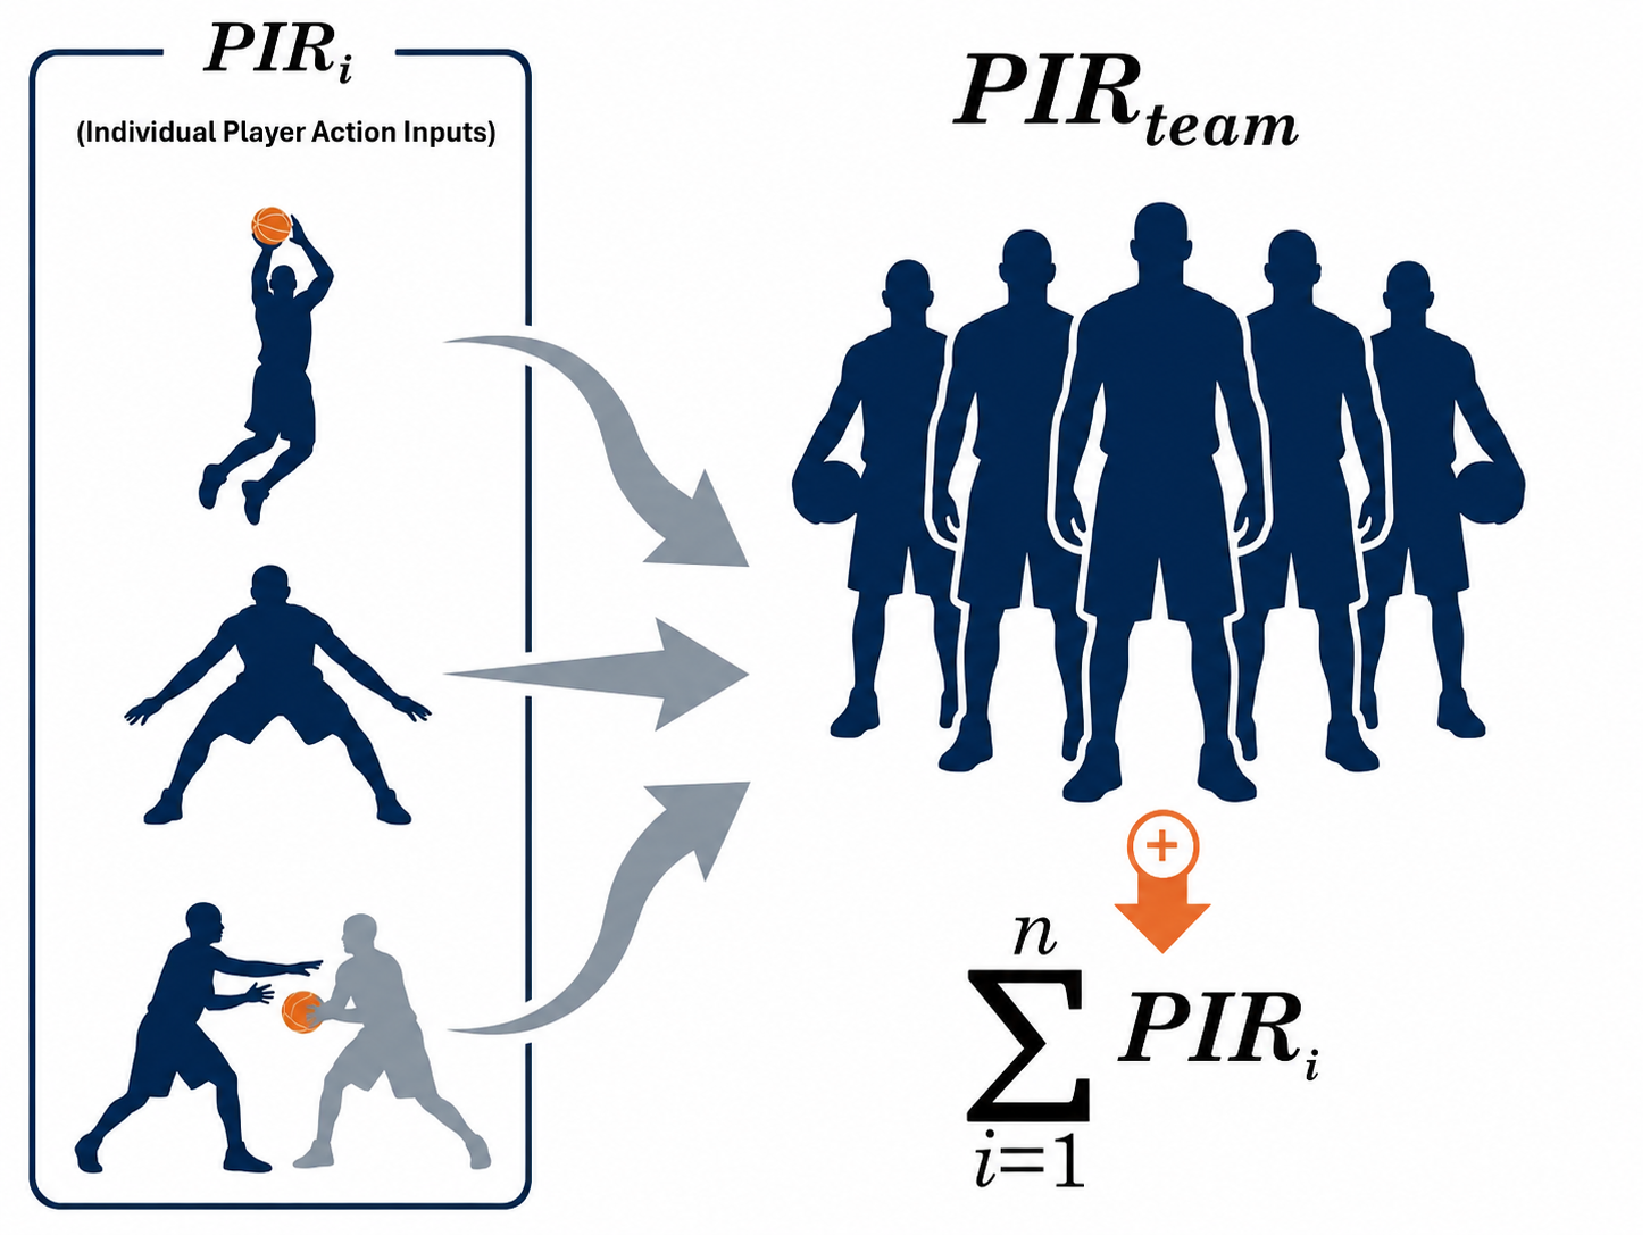
\includegraphics[width=.75\textwidth,trim=10bp 7bp 45bp 7bp,clip]{figures/PIR_team_diagram.pdf}
\caption{Existing official PIR construction. Player-attributed values sum to the player component of the official team ledger; team-only recorded actions are represented explicitly by the residual in Equation~\ref{eq:s-additivity}. This schematic does not depict RM-PIR calibration.}
\label{fig:s-official}
\end{figure}

\begin{figure}[t]
\centering
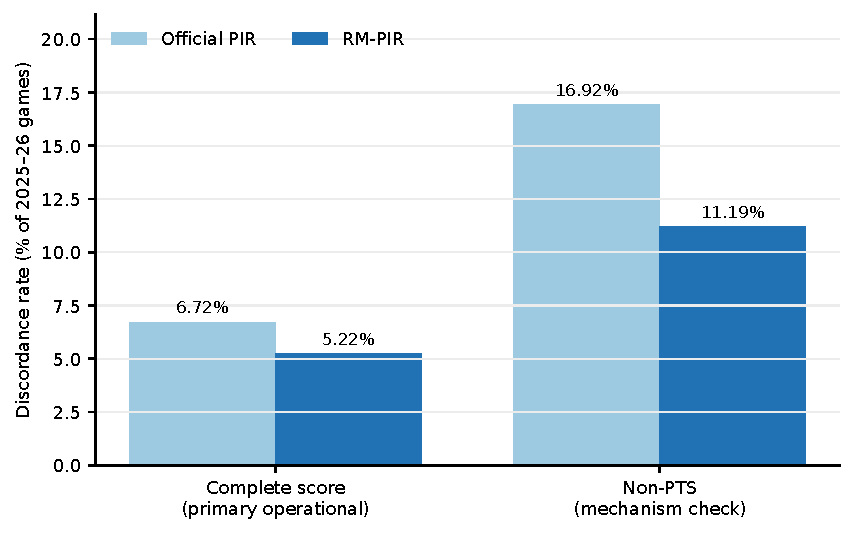
\includegraphics[width=.72\textwidth]{figures/vppir_validation.pdf}
\caption{2025--26 discordance rates for the complete-score primary outcome and nonpoint mechanism analysis. Discordance includes exact numerical ties and loser-higher games.}
\label{fig:s-validation}
\end{figure}

Under a common 0.5-unit equivalence band, 2025--26 complete-score W/T/L counts were 375/3/24 for official PIR and 378/4/20 for RM-PIR. For the nonpoint score they were 334/14/54 and 352/10/40. Thus the direction of the result did not depend on treating a numerically continuous RM-PIR score as having fewer exact ties than the integer-valued official score.

\subsection{Sensitivity summary}

\begin{table}[t]
\caption{Summary of 2025--26 sensitivity results. Ranges are signed RM-PIR minus official discordance changes in percentage points; negative values favour RM-PIR.}
\label{tab:s-sensitivity}
\centering
\small
\begin{tabular}{@{}p{0.52\textwidth}rr@{}}
\toprule
Sensitivity family & Nonpoint range & Complete range \\
\midrule
Seventeen primary/design configurations & -6.97 to -2.24 & -1.99 to -0.50 \\
Leave-one-target-club-out evaluations & -6.70 to -4.67 & -2.20 to -1.10 \\
Six post-fit scale conventions & -5.72 to -5.72 & -1.74 to -1.24 \\
Club-membership bootstrap, 95\% interval & -11.14 to -0.84 & -4.66 to 1.49 \\
Joint coefficient/club bootstrap, 95\% interval & -11.48 to -1.90 & -4.55 to 1.62 \\
\bottomrule
\end{tabular}
\end{table}

The 17 design configurations comprised wider raw bounds; one- and two-season windows; an expanded \(\tau/\alpha\) grid; multi-cutoff forward selection; overtime exclusion; 70-possession calibration contrasts; unrestricted block and foul groups; centred-SD and mean-absolute scale anchors; leave-one-calibration-season-out fits; regular-season-only evaluation; and exclusion of team-only residuals. The nonpoint change remained negative in every configuration. Boundary-active coefficients and the more variable complete-score scale response are retained as limitations, not treated as evidence of exact action values.

\section{Detailed 2025--26 team rankings}

The regular season provides an equal-exposure comparison because every club played 38 games. Total and per-game rankings are therefore identical. The all-stage table is reported separately because postseason participation changes cumulative opportunity.

\begin{table}[t]
\caption{2025--26 regular-season team rankings. Rank change is official rank minus RM-PIR rank; positive values denote upward movement.}
\label{tab:s-team-regular}
\centering
\tiny
\setlength{\tabcolsep}{1.5pt}
\begin{tabular}{@{}lrrrrrrrr@{}}
\toprule
Team & GP & PIR total & RM total & PIR/game & RM/game & PIR rank & RM rank & Change \\
\midrule
Olympiacos & 38 & 4164 & 3859.92 & 109.58 & 101.58 & 1 & 1 & 0 \\
Monaco & 38 & 4036 & 3773.86 & 106.21 & 99.31 & 2 & 2 & 0 \\
Real & 38 & 3957 & 3724.25 & 104.13 & 98.01 & 3 & 3 & 0 \\
Valencia & 38 & 3921 & 3675.93 & 103.18 & 96.74 & 4 & 4 & 0 \\
Zalgiris & 38 & 3771 & 3547.25 & 99.24 & 93.35 & 6 & 5 & +1 \\
Dubai & 38 & 3737 & 3545.84 & 98.34 & 93.31 & 9 & 6 & +3 \\
Maccabi & 38 & 3803 & 3539.55 & 100.08 & 93.15 & 5 & 7 & -2 \\
Panathinaikos & 38 & 3769 & 3535.72 & 99.18 & 93.05 & 7 & 8 & -1 \\
Hapoel Tel Aviv & 38 & 3753 & 3528.64 & 98.76 & 92.86 & 8 & 9 & -1 \\
Crvena Zvezda & 38 & 3714 & 3480.16 & 97.74 & 91.58 & 10 & 10 & 0 \\
Milan & 38 & 3671 & 3409.86 & 96.61 & 89.73 & 11 & 11 & 0 \\
Baskonia & 38 & 3626 & 3362.99 & 95.42 & 88.50 & 12 & 12 & 0 \\
Paris & 38 & 3531 & 3344.34 & 92.92 & 88.01 & 14 & 13 & +1 \\
Barcelona & 38 & 3558 & 3342.08 & 93.63 & 87.95 & 13 & 14 & -1 \\
Virtus & 38 & 3376 & 3136.22 & 88.84 & 82.53 & 15 & 15 & 0 \\
Fenerbahce & 38 & 3283 & 3105.13 & 86.39 & 81.71 & 17 & 16 & +1 \\
Partizan & 38 & 3287 & 3094.08 & 86.50 & 81.42 & 16 & 17 & -1 \\
Bayern & 38 & 3260 & 3053.61 & 85.79 & 80.36 & 18 & 18 & 0 \\
Anadolu Efes & 38 & 3239 & 2992.09 & 85.24 & 78.74 & 19 & 19 & 0 \\
ASVEL & 38 & 3052 & 2825.16 & 80.32 & 74.35 & 20 & 20 & 0 \\
\bottomrule
\end{tabular}
\end{table}

\begin{figure}[t]
\centering
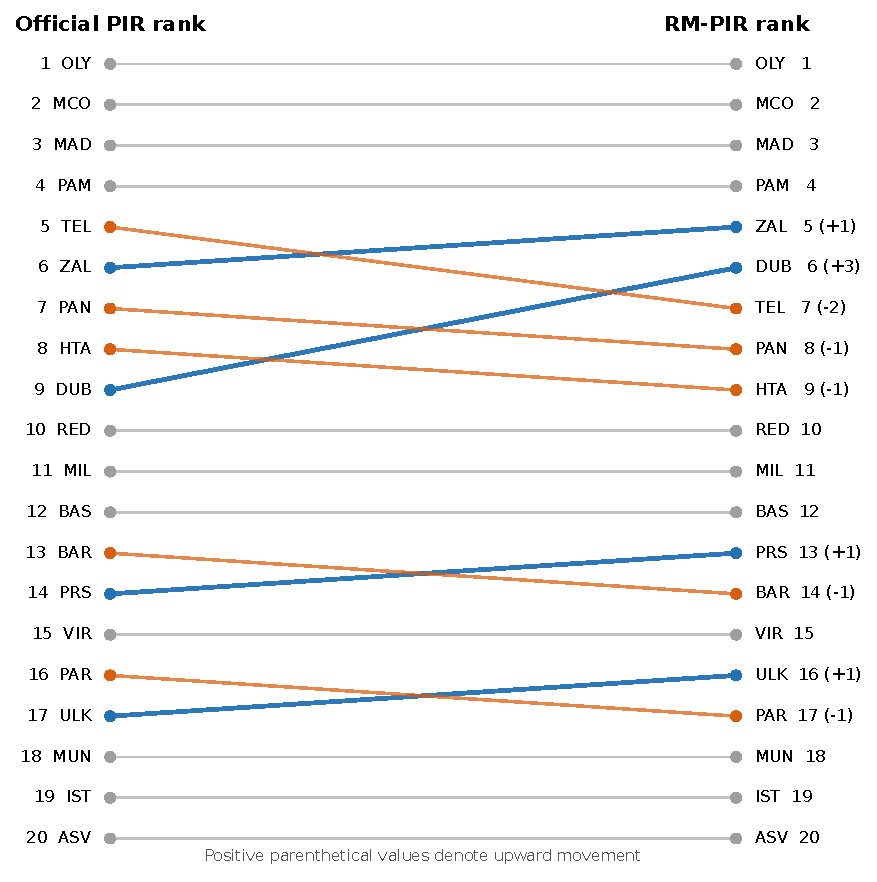
\includegraphics[width=.78\textwidth]{figures/vppir_team_rank_movement.pdf}
\caption{Regular-season rank movement from official PIR to RM-PIR. Rank one is shown at the top; positive changes represent upward movement under RM-PIR.}
\label{fig:s-team-ranks}
\end{figure}

\begin{table}[t]
\caption{2025--26 all-stage team rankings. Cumulative ranks reflect both scoring performance and unequal postseason opportunity; games played range from 38 to 44.}
\label{tab:s-team-all}
\centering
\tiny
\setlength{\tabcolsep}{1.5pt}
\begin{tabular}{@{}lrrrrrrrr@{}}
\toprule
Team & GP & PIR total & RM total & PIR/game & RM/game & PIR rank & RM rank & Change \\
\midrule
Olympiacos & 43 & 4727 & 4407.00 & 109.93 & 102.49 & 1 & 1 & 0 \\
Real & 44 & 4560 & 4305.12 & 103.64 & 97.84 & 2 & 2 & 0 \\
Valencia & 44 & 4550 & 4264.68 & 103.41 & 96.92 & 3 & 3 & 0 \\
Monaco & 43 & 4424 & 4126.15 & 102.88 & 95.96 & 4 & 4 & 0 \\
Panathinaikos & 44 & 4294 & 4045.57 & 97.59 & 91.94 & 5 & 5 & 0 \\
Zalgiris & 42 & 4114 & 3859.68 & 97.95 & 91.90 & 6 & 6 & 0 \\
Hapoel Tel Aviv & 42 & 4087 & 3840.48 & 97.31 & 91.44 & 7 & 7 & 0 \\
Dubai & 38 & 3737 & 3545.84 & 98.34 & 93.31 & 10 & 8 & +2 \\
Crvena Zvezda & 39 & 3780 & 3542.76 & 96.92 & 90.84 & 9 & 9 & 0 \\
Maccabi & 38 & 3803 & 3539.55 & 100.08 & 93.15 & 8 & 10 & -2 \\
Fenerbahce & 43 & 3720 & 3512.44 & 86.51 & 81.68 & 12 & 11 & +1 \\
Barcelona & 40 & 3726 & 3502.92 & 93.15 & 87.57 & 11 & 12 & -1 \\
Milan & 38 & 3671 & 3409.86 & 96.61 & 89.73 & 13 & 13 & 0 \\
Baskonia & 38 & 3626 & 3362.99 & 95.42 & 88.50 & 14 & 14 & 0 \\
Paris & 38 & 3531 & 3344.34 & 92.92 & 88.01 & 15 & 15 & 0 \\
Virtus & 38 & 3376 & 3136.22 & 88.84 & 82.53 & 16 & 16 & 0 \\
Partizan & 38 & 3287 & 3094.08 & 86.50 & 81.42 & 17 & 17 & 0 \\
Bayern & 38 & 3260 & 3053.61 & 85.79 & 80.36 & 18 & 18 & 0 \\
Anadolu Efes & 38 & 3239 & 2992.09 & 85.24 & 78.74 & 19 & 19 & 0 \\
ASVEL & 38 & 3052 & 2825.16 & 80.32 & 74.35 & 20 & 20 & 0 \\
\bottomrule
\end{tabular}
\end{table}

\section{Secondary player analyses}

The 2025--26 locked team coefficients were applied uniformly to player rows. Players with at least one positive-minute appearance were aggregated by stable official player identifier; players appearing for multiple clubs were counted once. The resulting 335-player table is supplied as the machine-readable Supplementary Table S7. It contains games, minutes, official PIR and RM-PIR season totals, competition ranks and rank changes. This table describes alternative allocations of the recorded ledger and is not a ranking of causal impact.

Across 8,741 positive-minute player-games, raw Spearman correlations with official on-court plus-minus were 0.3012 for official PIR and 0.3186 for RM-PIR. Rank-based partial correlations controlling minutes were 0.2792 and 0.2941; controlling estimated possession exposure, they were 0.2795 and 0.2942. The latter difference was 0.0147 (whole-game bootstrap 95\% interval, 0.0092 to 0.0205). These are small convergent associations with a context-dependent comparator, not validation of individual credit.

Current-game association with team-margin-residualised on-court plus-minus in the next appearance was 0.0228 for official PIR and 0.0195 for RM-PIR; association with the mean over exactly the next three appearances was 0.0347 and 0.0300. The near-zero estimates provide no evidence that the team-calibrated RM-PIR score improves short-horizon player outcome association. A genuine adjusted-plus-minus analysis was not attempted because the analysis-ready data contain no lineup-stint design matrix. Player-level claims in the main paper are limited accordingly.

\section{Supplementary data inventory}

The reproducibility package contains the following machine-readable supplementary material:

\begin{itemize}
\item complete season/game eligibility and exclusion register;
\item rolling target-level W/T/L classifications and paired transitions;
\item annual locked coefficients, scale factors and optimisation diagnostics;
\item conditional coefficient-bootstrap intervals and boundary frequencies;
\item all 20 regular-season and all-stage team rankings;
\item all 335 eligible player totals and ranks (Supplementary Table S7);
\item additivity residuals at component and team-game levels;
\item tie, scale, pace, window, bound, grouping and dependence sensitivities; and
\item the analysis-decision provenance table and deterministic output manifest.
\end{itemize}

\bibliography{bibliography}

\end{document}
